%!TEX root = ../main.tex

\ParteEsercizi

Richiami

VA: Sia $(\Omega ,\mathcal{A} ,\PP)$ uno spazio di probabilità. Una funzione $X:(\Omega ,\mathcal{A})\rightarrow (\mathbb{R} ,\mathcal{B})$ si dice variabile aleatoria reale se è misurabile, i.e. $\forall B\in \mathcal{B} ,X^{-1}(B) \in \mathcal{A}$.

LEGGE: la legge di una variabile aleatoria reale $X$ è la misura di probabilità $P^{X}(B) =\PP(X\in B) =\PP\left(X^{-1}(B)\right) =\PP(\{\omega \in \Omega :X(\omega) \in B\})$, $\forall B\in \mathcal{B}$.
\begin{oss}
	La legge è univocamente determinata dalla funzione di ripartizione, ossia $F:\mathbb{R}\rightarrow \mathbb{R}$ tale che $F(t) =\PP(X\leq t) =P^{X}((-\infty ,t])$. La funzione di ripartizione è definita su tutto $\mathbb{R}$ e si definisce solo per le VA reali.
\end{oss}
\begin{oss}
Somme, prodotti, limiti di VA reali sono VA reali.
\end{oss}
Funzioni boreliane: una funzione $f:(\mathbb{R} ,\mathcal{B})\rightarrow (\mathbb{R} ,\mathcal{B})$ si dice boreliana se è misurabile.
\begin{oss}
Sono boreliane le funzioni continue e generalmente continue (i.e. continue a tratti).
\end{oss}
\begin{oss}
Composizione di VA reali con funzioni boreliane sono VA reali.
\end{oss}
VA discrete: una VA reale $X$ si dice \textbf{discreta} se assume con probabilità $1$ valori in un insieme $S$ al più numerabile $\PP(X\in S) =1$. $\iff $Una VA reale $X$ si dice discreta se e solo se $P^{X}$ è discreta, ossia $\exists S\subset \mathbb{R}$ al più numerabile e $p_{X} :S\rightarrow [0,1]$ tale che $P^{X}(B) =\sum\limits_{x\in B\cap S} p_{X}(x)$, $\forall B\in \mathcal{B}$.

La funzione $p_{X}$ si dice \textbf{densità discreta} di $X$. Si dice \textbf{supporto} di $P^{X}$ l'insieme $S_{X} =\{x\in \mathbb{R} :p_{X}(x)  >0\}$.
\begin{oss}
Posso, ma non per forza, pensare $S=S_{X}$.
\end{oss}
Graficamente


\tikzset{every picture/.style={line width=0.75pt}} %set default line width to 0.75pt        

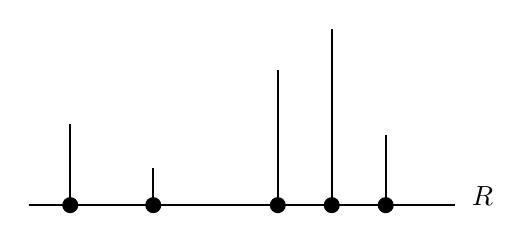
\begin{tikzpicture}[x=0.75pt,y=0.75pt,yscale=-1,xscale=1]
%uncomment if require: \path (0,132); %set diagram left start at 0, and has height of 132

%Straight Lines [id:da6279508270671126] 
\draw    (178,114) -- (383.5,114) ;
%Straight Lines [id:da5575359122441383] 
\draw    (198,114) -- (198,75) ;
\draw [shift={(198,114)}, rotate = 270] [color={rgb, 255:red, 0; green, 0; blue, 0 }  ][fill={rgb, 255:red, 0; green, 0; blue, 0 }  ][line width=0.75]      (0, 0) circle [x radius= 3.35, y radius= 3.35]   ;
%Straight Lines [id:da6000000943512647] 
\draw    (238,114) -- (238,96) ;
\draw [shift={(238,114)}, rotate = 270] [color={rgb, 255:red, 0; green, 0; blue, 0 }  ][fill={rgb, 255:red, 0; green, 0; blue, 0 }  ][line width=0.75]      (0, 0) circle [x radius= 3.35, y radius= 3.35]   ;
%Straight Lines [id:da5096851903596566] 
\draw    (298,114) -- (298,49) ;
\draw [shift={(298,114)}, rotate = 270] [color={rgb, 255:red, 0; green, 0; blue, 0 }  ][fill={rgb, 255:red, 0; green, 0; blue, 0 }  ][line width=0.75]      (0, 0) circle [x radius= 3.35, y radius= 3.35]   ;
%Straight Lines [id:da19644762271772676] 
\draw    (324,114) -- (324,29) ;
\draw [shift={(324,114)}, rotate = 270] [color={rgb, 255:red, 0; green, 0; blue, 0 }  ][fill={rgb, 255:red, 0; green, 0; blue, 0 }  ][line width=0.75]      (0, 0) circle [x radius= 3.35, y radius= 3.35]   ;
%Straight Lines [id:da9962709356508239] 
\draw    (350,114) -- (350,80) ;
\draw [shift={(350,114)}, rotate = 270] [color={rgb, 255:red, 0; green, 0; blue, 0 }  ][fill={rgb, 255:red, 0; green, 0; blue, 0 }  ][line width=0.75]      (0, 0) circle [x radius= 3.35, y radius= 3.35]   ;

% Text Node
\draw (390,103.4) node [anchor=north west][inner sep=0.75pt]    {$\mathbb{R}$};


\end{tikzpicture}

\begin{oss}
Se $X$ è VA reale con funzione di ripartizione $F_{X}$ costante a tratti, allora $X$ è discreta. $S$ sarà l'insieme dei punti di discontinuità e $p_{X}$ l'ampiezza dei salti.
\end{oss}
Esempio. Sia $X$ la VA che indica il numero di teste ottenute in un lancio di $3$ monete non truccate. Si può calcolare
\begin{equation*}
\PP(X\leq x) =F_{X}(x) =
\begin{cases}
0 & \text{se} \ x< 0\\
\frac{1}{8} & \text{se} \ 0\leq x< 1\\
\frac{1}{2} & \text{se} \ 1\leq x< 2\\
\frac{7}{8} & \text{se} \ 2\leq x< 3\\
1 & \text{se} \ x\geq 3
\end{cases}
\end{equation*}

\tikzset{every picture/.style={line width=0.75pt}} %set default line width to 0.75pt        

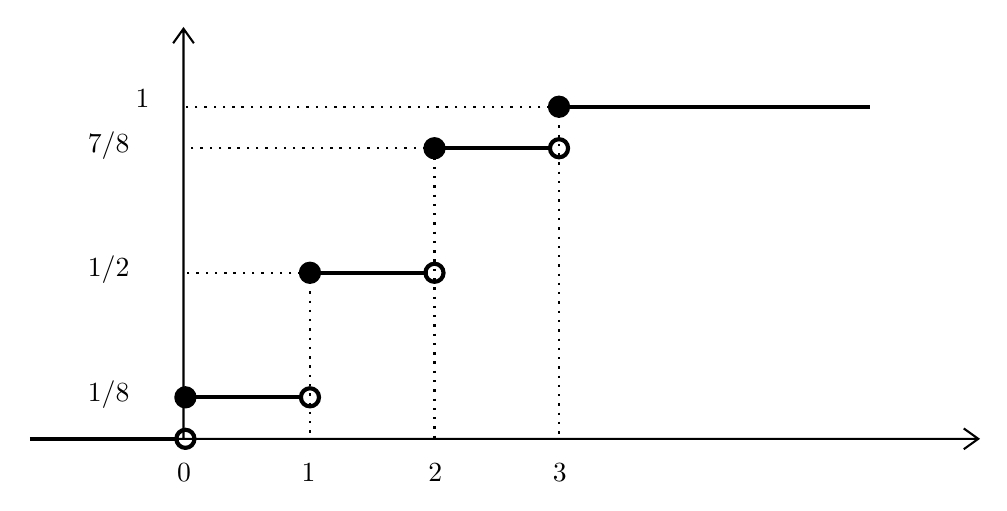
\begin{tikzpicture}[x=0.75pt,y=0.75pt,yscale=-1,xscale=1]
%uncomment if require: \path (0,266); %set diagram left start at 0, and has height of 266

%Shape: Axis 2D [id:dp7785871975299155] 
\draw  (80,221.59) -- (531.5,221.59)(148.58,24) -- (148.58,221.59) (524.5,216.59) -- (531.5,221.59) -- (524.5,226.59) (143.58,31) -- (148.58,24) -- (153.58,31)  ;
%Straight Lines [id:da18293161685682802] 
\draw [line width=1.5]    (149.5,201.59) -- (206.15,201.59) ;
\draw [shift={(209.5,201.59)}, rotate = 0] [color={rgb, 255:red, 0; green, 0; blue, 0 }  ][line width=1.5]      (0, 0) circle [x radius= 4.36, y radius= 4.36]   ;
\draw [shift={(149.5,201.59)}, rotate = 0] [color={rgb, 255:red, 0; green, 0; blue, 0 }  ][fill={rgb, 255:red, 0; green, 0; blue, 0 }  ][line width=1.5]      (0, 0) circle [x radius= 4.36, y radius= 4.36]   ;
%Straight Lines [id:da48480951914110326] 
\draw [line width=1.5]    (209.5,141.59) -- (266.15,141.59) ;
\draw [shift={(269.5,141.59)}, rotate = 0] [color={rgb, 255:red, 0; green, 0; blue, 0 }  ][line width=1.5]      (0, 0) circle [x radius= 4.36, y radius= 4.36]   ;
\draw [shift={(209.5,141.59)}, rotate = 0] [color={rgb, 255:red, 0; green, 0; blue, 0 }  ][fill={rgb, 255:red, 0; green, 0; blue, 0 }  ][line width=1.5]      (0, 0) circle [x radius= 4.36, y radius= 4.36]   ;
%Straight Lines [id:da7961634069824368] 
\draw [line width=1.5]    (329.5,61.59) -- (479.5,61.59) ;
\draw [shift={(329.5,61.59)}, rotate = 0] [color={rgb, 255:red, 0; green, 0; blue, 0 }  ][fill={rgb, 255:red, 0; green, 0; blue, 0 }  ][line width=1.5]      (0, 0) circle [x radius= 4.36, y radius= 4.36]   ;
%Straight Lines [id:da8883646431391186] 
\draw [line width=1.5]    (269.5,81.59) -- (326.15,81.59) ;
\draw [shift={(329.5,81.59)}, rotate = 0] [color={rgb, 255:red, 0; green, 0; blue, 0 }  ][line width=1.5]      (0, 0) circle [x radius= 4.36, y radius= 4.36]   ;
\draw [shift={(269.5,81.59)}, rotate = 0] [color={rgb, 255:red, 0; green, 0; blue, 0 }  ][fill={rgb, 255:red, 0; green, 0; blue, 0 }  ][line width=1.5]      (0, 0) circle [x radius= 4.36, y radius= 4.36]   ;
%Straight Lines [id:da7731345693466043] 
\draw [line width=1.5]    (74.5,221.59) -- (146.15,221.59) ;
\draw [shift={(149.5,221.59)}, rotate = 0] [color={rgb, 255:red, 0; green, 0; blue, 0 }  ][line width=1.5]      (0, 0) circle [x radius= 4.36, y radius= 4.36]   ;
%Straight Lines [id:da8859133785362521] 
\draw  [dash pattern={on 0.84pt off 2.51pt}]  (209.5,141.59) -- (209.5,221.5) ;
%Straight Lines [id:da7507588586070726] 
\draw  [dash pattern={on 0.84pt off 2.51pt}]  (269.5,81.59) -- (269.5,221.5) ;
%Straight Lines [id:da9788753181983849] 
\draw  [dash pattern={on 0.84pt off 2.51pt}]  (329.5,61.59) -- (329.5,221.5) ;
%Straight Lines [id:da37404258980558325] 
\draw  [dash pattern={on 0.84pt off 2.51pt}]  (209.5,141.59) -- (150.5,141.59) ;
%Straight Lines [id:da8671546504037952] 
\draw  [dash pattern={on 0.84pt off 2.51pt}]  (269.5,81.59) -- (150.5,81.59) ;
%Straight Lines [id:da178027804620988] 
\draw  [dash pattern={on 0.84pt off 2.51pt}]  (329.5,61.59) -- (149.5,61.59) ;

% Text Node
\draw (101,191.9) node [anchor=north west][inner sep=0.75pt]    {$1/8$};
% Text Node
\draw (101,131.9) node [anchor=north west][inner sep=0.75pt]    {$1/2$};
% Text Node
\draw (101,71.9) node [anchor=north west][inner sep=0.75pt]    {$7/8$};
% Text Node
\draw (124,51.9) node [anchor=north west][inner sep=0.75pt]    {$1$};
% Text Node
\draw (204,231.9) node [anchor=north west][inner sep=0.75pt]    {$1$};
% Text Node
\draw (144,231.9) node [anchor=north west][inner sep=0.75pt]    {$0$};
% Text Node
\draw (325,231.9) node [anchor=north west][inner sep=0.75pt]    {$3$};
% Text Node
\draw (265,231.9) node [anchor=north west][inner sep=0.75pt]    {$2$};


\end{tikzpicture}

$S$ è l'insieme dei punti di discontinuità di $F$: infatti la VA assume i valori in $S=\{0,1,2,3\}$.

$p_{X}(x) =\PP(X=x)$, per esempio $p_{X}(2) =\PP(X=2) =F_{X}(2) -F_{X}(2)^{-} =\frac{7}{8} -\frac{1}{2} =\frac{3}{8}$ che è l'ampiezza del salto da $1$ a $2$, i.e. $p_{X}(x)$ rappresenta l'ampiezza dei salti.
\begin{oss}
$\Omega \ \text{discreto} \implies \mathrm{Im}(X) \ \text{discreta} \implies X\ \text{discreta} .$
\end{oss}
Possiamo riassumere quanto detto sopra nella seguente
\begin{theorem}
Sia $X:\Omega \rightarrow S\subset \mathbb{R}$ una VA discreta che assume, con probabilità $1$, valori in $S=\{x_{k} :k\in I\}$, $I\subset \mathbb{Z}$. Allora
\end{theorem}
\begin{enumerate}
\item $0\leq p_{X}(x) \leq 1,\forall x\in \mathbb{R}$ e $p_{X}(x) =0,\forall x\notin S$
\item $\sum\limits_{k\in I} p_{X}(k) =1$
\item se $F_{X}$ è la funzione di ripartizione di $X$ allora
\begin{equation*}
F_{X}(x) =\sum\limits_{k:x_{k} \leq x} p_{X}(x_{k}) ,\ \ \ \ \forall x\in \mathbb{R}
\end{equation*}
\item se i punti di $S$ possono essere numerati in modo tale che $x_{h} < x_{k}$ se $h< k$, allora
\begin{equation*}
p_{X}(x_{k}) =F_{X}(x_{k}) -F_{X}(x_{k-1}) ,\ \ \ \ \forall k\in I
\end{equation*}
\item se $B\subset \mathbb{R}$ allora
\begin{equation*}
\PP(X\in B) =\sum\limits_{k:x_{k} \in B} p_{X}(x_{k})
\end{equation*}
\end{enumerate}
\begin{oss}
$(3)$ e $(4)$ ci dicono che: se i punti di $S$ possono essere numerati in modo tale che $x_{h} < x_{k}$ per $h< k$, allora la funzione di ripartizione di una VA discreta è una funzione a gradini, che i gradini sono situati nei punti dell'insieme $S$ (i.e. $S$ è l'insieme dei punti di discontinuità di $F_{X}$) e che l'altezza del gradino corrispondente al punto $x_{k} \in S$ è proprio $p_{X}(x_{k})$ (i.e. $p_{X}$ è l'ampiezza dei salti della funzione di ripartizione $F_{X}$ nei punti di discontinuità).

$(5)$ ci dice che è possibile costruire la probabilità di ogni evento $B\in \mathcal{A}$ a partire dalla densità di probabilità $p_{X}$.
\end{oss}

\Esercizio{fatto}

Si consideri la probabilità uniforme nell'intervallo $[0,1$] su $(\mathbb{R} ,\mathcal{B})$. Qui si definiscano le funzioni
\begin{itemize}
\item $X(\omega) =\Ind_{[0,p]}(\omega) ,\ \omega \in \mathbb{R} ,$
\item $Y(\omega) =\Ind_{[0,p]}(\omega) +\omega \Ind_{(-\infty ,0) \cup (1,\infty)}(\omega) ,\ \omega \in \mathbb{R} ,$
\end{itemize}

dove $0< p< 1$ è un parametro fissato. Si ricordi che la notazione $\Ind_{A}$ indica la funzione indicatrice dell'insieme $A\in \mathcal{B}$, ossia
\begin{equation*}
\Ind_{A}(\Omega) \coloneqq
\begin{cases}
1,\ \omega \in A,\\
0,\ \omega \notin A,
\end{cases}
\ \omega \in \mathbb{R} .
\end{equation*}
\begin{enumerate}
\item Si mostri che $X$ e $Y$ sono variabili aleatorie reali discrete. Si dimostri inoltre che $X=Y$ q.c.
\item Si determinino legge $P^{X} ,P^{Y}$ e valore atteso $\EE[X] ,\EE[Y]$.
\item Si esibisca un'altra variabile aleatoria $X' $ con la stessa legge di $X$, ma definita su uno spazio $\Omega ' $ discreto.
\end{enumerate}

\Esercizio{}

Sia $\Omega =[0,1]$ e si consideri la $\sigma $-algebra di Borel $A=\mathcal{B}([0,1])$. Si definisca $\PP$ la probabilità uniforme su $(\Omega ,\mathcal{A})$, caratterizzata dalla proprietà:
\begin{equation*}
\PP((a,b]) =b-a,\ \text{per ogni} \ a< b,\ \text{con} \ a,b\in [0,1] .
\end{equation*}
\begin{enumerate}
\item Provare che $\PP([a,b]) =\PP([a,b)) =\PP((a,b)) =b-a$ per ogni $a< b$, con $a,b\in [0,1]$.
\item Mostrare che $\PP(\{\Omega \}) =0$ per ogni $\omega \in \Omega $.
\end{enumerate}

Si definiscano le seguenti funzioni, per ogni $\omega \in \Omega $
\begin{equation*}
X(\omega) \ =\ \Ind_{[0,p]}(\omega) ,\ \ \ \ Y(\omega) =\Ind_{(0,p)}(\omega) ,\ \ \ \ Z(\omega) =\Ind_{[0,p]}(\omega) +\Ind_{J}(\omega) ,
\end{equation*}
dove $0< p< 1$ è un parametro fissato e $J=\left\{\frac{1}{n}\right\}_{n\in \mathbb{N}} =\left\{1,\frac{1}{2} ,\frac{1}{3} ,\dots \right\}$.
\begin{enumerate}
\item Si mostri che $X$, $Y$ e $Z$ sono variabili aleatorie reali discrete. Si dimostri inoltre che $X=Y=Z$ q.c.
\item Si determinino legge $P^{X} ,P^{Y} ,P^{Z}$ e valore atteso $\EE[X] ,\EE[Y] ,\EE[Z]$.
\end{enumerate}

\Esercizio{}

Si consideri la funzione reale di variabile reale
\begin{equation*}
F(x) =
\begin{cases}
0, & x< 0,\\
1/2, & 0\leq x< 1,\\
2/3, & 1\leq x< \ 2,\\
11/12, & 2\leq x< \ 3,\\
1, & x\geq 3.
\end{cases}
\end{equation*}
\begin{enumerate}
\item Si mostri che $F$ è la funzione di ripartizione di una probabilità $\PP$ su $(\mathbb{R} ,\mathcal{B})$.
\item Si mostri che $\PP$ è una probabilità discreta su $(\mathbb{R} ,\mathcal{B})$, trovando i punti $x_{k}$ dove $\PP$ è concentrata e le corrispondenti probabilità $p_{k}$, o equivalentemente determinando la densità (discreta) $p:\mathbb{R}\rightarrow [0,1]$ definita come segue:
\begin{equation*}
p(x) =P(\{x\}) =
\begin{cases}
p_{k} & \text{se} \ x=x_{k}\\
0 & \text{altrimenti}
\end{cases}
\end{equation*}
per ogni $x\in \mathbb{R}$.
\item Quanto valgono $\PP((1/2,+\infty)) ,\PP((2,4]) ,\PP((1,2)) ,\PP((-\infty ,3))$?
\item Si introduca una variabile aleatoria reale e discreta $X$ di legge $P$, definita su uno spazio $\Omega $ \textit{discreto}.
\item Si introduca una variabile aleatoria reale e discreta $X$ di legge $P$, definita su uno spazio $\Omega $ \textit{continuo}.
\item Determinare la densità discreta di $X$, il suo valore atteso e la sua varianza.
\item Determinare la probabilità degli eventi: $X >\frac{1}{2} ,2< X\leq 4,1< X< 2$ e $X< 3$.
\item Determinare i quartili di $X$.
\item Mostrare che $Y=(X-2)^{2}$ è una variabile aleatoria discreta. Determinarne legge e valore atteso.
\end{enumerate}

\Esercizio{}

Si consideri la funzione
\begin{equation*}
F(x) =\sum\limits_{i=1}^{+\infty }\frac{1}{2^{i}}\Ind_{\left[\frac{1}{i} ,+\infty \right)}(x) ,\ \ \ \ x\in \mathbb{R}
\end{equation*}
\begin{enumerate}
\item Si mostri che si tratta di una funzione di ripartizione.
\end{enumerate}

Sia dunque $X$ una variabile aleatoria discreta con funzione di ripartizione $F$.
\begin{enumerate}
\item Determinare la densità discreta di $X$.
\item 3. Determinare la probabilità dei seguenti eventi:
\begin{enumerate}
\item $X\geq 1$;
\item $X\geq 1$;
\item $X\leq 0$;
\item $0\leq X< \frac{1}{2}$.
\end{enumerate}
\end{enumerate}

\Esercizio{fatto}

Consideriamo infinite prove di Bernoulli indipendenti con probabilità di successo $0< p< 1$. Sia quindi $\Omega =\{0,1\}^{\mathbb{N}}$, sia $\mathcal{A} =\sigma (E_{k} \ |\ k=1,2,\dots)$ con
\begin{equation*}
E_{k} =\text{successo alla prova} \ k,
\end{equation*}
e sia $\PP$ tale che $\{E_{k}\}_{k\in \mathbb{N}}$ risulti una famiglia di eventi indipendenti con $\PP(E_{k}) =p$ per ogni $k$. Indicato con $\omega =(\omega_{k})_{k=1}^{\infty }$ il generico esito dello spazio campionario $\Omega $, definiamo le funzioni
\begin{equation*}
X_{n} :\Omega \rightarrow \mathbb{R} ,\ \ \ \ X_{n}(\omega) =\omega_{n} ,\ \ \ \ n\in \mathbb{N} .
\end{equation*}
\begin{enumerate}
\item Si mostri che $X_{n} =\Ind_{E_{n}}$.
\item Si mostri che le $X_{n}$ sono variabili aleatorie reali discrete e se ne interpreti il significato probabilistico.
\item Si determini la legge delle $X_{n}$.
\item Per ogni $n$, si mostri che $Y_{n} =\sum_{k=1}^{n} X_{k}$ è una variabile aleatoria discreta, se ne dia il significato probabilistico e se ne determini la legge.
\item Si mostri che $Z=\min\{n\in \mathbb{N} :X_{n} =1\} =$ \event{numero di prove necessarie per il primo successo}, con la convenzione $\min \emptyset =+\infty $, è una variabile aleatoria discreta e se ne calcoli la legge.
\item Si mostri che $W=$ \event{numero di insuccessi prima del primo successo} è una variabile aleatoria discreta e se ne calcoli la legge.
\item Si mostri che $V=\liminf\limits_{n} X_{n}$ e $U=\limsup\limits_{n} X_{n}$ sono variabili aleatorie discrete e se ne calcolino le leggi.
\end{enumerate}

Cosa sarebbe cambiato se avessimo realizzato in un altro spazio di probabilità $(\Omega ' ,\mathcal{A} ' ,\PP ')$, diverso dallo spazio di Bernoulli, una successione di eventi $E_{n} ' $ indipendenti e tali che $\PP ' (E_{n} ') =p$, ed avessimo poi posto $X_{n} ' =\Ind_{E_{n} ' }$, ovvero se avessimo usato un differente spazio di probabilità per rappresentare infinite prove di Bernoulli indipendenti con probabilità di successo $0< p< 1$?

\Esercizio{$\star$}

Sia $X$ una variabile aleatoria a valori in $\{0,1,2,\dots \}$. Si mostri che
\begin{equation*}
\EE[X] =\sum\limits_{n=0}^{\infty }\PP(X >n) .
\end{equation*}

\Esercizio{(Distribuzione binomiale). fatto}

Si consideri una variabile aleatoria binomiale $X$ di parametri $n$ e $p$, con $n\in \mathbb{N}$ e $0< p< 1$. Scriviamo $X\sim B(n,p)$.
\begin{enumerate}
\item Calcolare il valore atteso $\EE[X]$.
\item Calcolare la varianza di $X$.
\item Calcolare le mode di $X$, ovvero i punti di massimo della densità discreta di $X$.
\end{enumerate}

\Esercizio{(Distribuzione di Poisson). fatto}

Si consideri una variabile aleatoria di Poisson $X$ di parametro $\lambda  >0$. Scriviamo $X\sim P(\lambda)$.
\begin{enumerate}
\item Calcolare il valore atteso $\EE[X]$.
\item Calcolare la varianza di $X$.
\item Calcolare le mode di $X$.
\item Dato $k\in \{1,2,\dots \}$, quale $\lambda  >0$ massimizza $\PP(X=k)$?
\end{enumerate}

\Esercizio{(Distribuzione geometrica). fatto}

Si consideri $X\sim \mathcal{G}(p)$, variabile aleatoria geometrica di parametro $p$, $0< p< 1$. Si ha pertanto
\begin{equation*}
\PP(X=k) =p(1-p)^{k-1} ,\ \ \ \ k\in \mathbb{N} .
\end{equation*}
\begin{enumerate}
\item Mostrare due diversi spazi $(\Omega ,\mathcal{A} ,\PP)$, uno discreto e uno continuo, su cui è possibile definire $X$.
\item Calcolare le mode di $X$.
\item Calcolare la funzione di ripartizione $F$ di $X$.
\item Calcolare il valore atteso $\EE[X]$.
\item (Proprietà di assenza di memoria) Mostrare che $\PP(X >i+j\ |\ X >i) =\PP(X >j)$ per ogni $i,j\in \mathbb{N}$.
\item (*) Si inverta il risultato appena ottenuto: se $T$ è una variabile aleatoria reale discreta a valori in $\mathbb{N}$ tale che $\PP(T >i+j\ |\ T >i) =\PP(T >j)$ per ogni $i,j\in \mathbb{N}$, allora $T\sim \mathcal{G}(q$) con $q=\PP(T=1)$.
\end{enumerate}

\Esercizio{}

Data una variabile aleatoria $X$ di Poisson di media $3$, si considerino
\begin{equation*}
Y=\min(3,X) ,\ \ \ \ W=e^{X/3} .
\end{equation*}
\begin{enumerate}
\item Si mostri che $Y$ e $W$ sono variabili aleatorie reali e discrete.
\item Si calcolino le loro distribuzioni.
\item Si calcolino le loro medie.
\end{enumerate}

\Esercizio{}

Data una variabile aleatoria $X$ con distribuzione geometrica di media $3$, si considerino
\begin{equation*}
Y=\min(3,X) ,\ \ \ \ W=e^{X/3} .
\end{equation*}
\begin{enumerate}
\item Si mostri che $Y$ e $W$ sono variabili aleatorie reali e discrete.
\item Si calcolino le loro distribuzioni.
\item Si calcolino le loro medie.
\end{enumerate}

\Esercizio{fatto}

In una certa provincia montuosa si può supporre che il numero $X$ di frane al mese sia una variabile aleatoria con legge di Poisson di parametro $\lambda =2.3$.
\begin{enumerate}
\item Calcolare la probabilità che ci siano almeno due frane in un dato mese.
\item Calcolare mediana e quantile di ordine $0.6$ del numero di frane mensili.
\item Quanto dovrebbe valere il parametro $\lambda $ affinché la probabilità che in un mese non ci siano frane sia superiore a $1/2$?
\end{enumerate}

\Esercizio{}

Al buio cerco la chiave del mio ufficio in un mazzo di $10$ chiavi tutte della stessa fattura. Ovviamente metto da parte le chiavi provate. Sia $X$ il numero di chiavi che devo provare per aprire l'ufficio.
\begin{enumerate}
\item Qual è la legge di $X$?
\item Qual è il numero atteso di tentativi da fare?
\item Quanto vale la probabilità di controllare almeno $8$ chiavi?
\item Sapendo che al primo tentativo non ho trovato la chiave giusta, con quale probabilità non la trovo neanche al secondo?
\item Come cambiano le risposte ai punti precedenti se stupidamente non metto da parte le chiavi già provate prima di procedere a provarne una nuova?
\end{enumerate}

\Esercizio{}

Nel Gioco del Lotto ad ogni estrazione settimanale $5$ numeri vengono estratti simultaneamente da un'urna che contiene $90$ palline numerate da $1$ a $90$. Fissato un numero, ad esempio il $67$, sia $p$ la probabilità che esca in una singola estrazione.
\begin{enumerate}
\item Quanto vale p?
\item Qual è la probabilità che dopo $30$ estrazioni il $67$ non sia ancora uscito?
\item Supponiamo che nelle prime $100$ estrazioni il $67$ non sia ancora uscito, qual è la probabilità che esca dopo la $130$ esima estrazione?
\item Qual è la probabilità che esca almeno $6$ volte nelle prime $50$ estrazioni?
\item Se nelle prime $10$ estrazioni il $67$ è comparso $2$ volte, con quale probabilità è comparso alle prime $2$ estrazioni?
\end{enumerate}

\Esercizio{fatto}

Un'urna contiene una pallina rossa ed una blu. Una pallina viene estratta a caso. Se è blu il gioco termina. Se è rossa la pallina viene rimessa nell'urna insieme ad un'altra rossa.
\begin{enumerate}
\item Supponiamo che la procedura sopra descritta venga ripetuta fino ad aver fatto $10$ estrazioni o alla prima estrazione di una pallina blu, se si presenta prima della decima estrazione. Sia $X$ il numero di estrazioni effettuate. Determinare la distribuzione di $X$ e il suo valore atteso.
\item Supponiamo ora che il gioco termini solo quando compare la prima pallina blu e sia Y il numero di estrazioni in questo caso.
\begin{enumerate}
\item Determinare la probabilità di effettuare almeno n estrazioni prima che il gioco finisca.
\item Determinare la probabilità che il gioco non finisca mai.
\item Determinare la distribuzione di $Y$ e il suo valore atteso.
\end{enumerate}
\end{enumerate}

\Esercizio{fatto}

I punti $N$ realizzati dai Caprica Buccaneers in una partita di Piramid hanno distribuzione di Poisson di media $\lambda $. Vi propongono di scommettere contro i Caprica Buccaneers alla prossima partita: a fronte di una vostra puntata unitaria riceverete un ricavo pari a
\begin{equation*}
R=\frac{7}{3^{N}} ,
\end{equation*}
guadagnando quindi $G=R-1$.
\begin{enumerate}
\item Trovare la distribuzione del ricavo $R$ in funzione di $\lambda $.
\item Trovare il ricavo atteso in funzione di $\lambda $.
\end{enumerate}

Si supponga che la scommessa proposta sia equa.
\begin{enumerate}
\item Quanti punti a partita segnano mediamente i Caprica Buccaneers?
\item Con quale probabilità otterrete il ricavo massimo?
\item Con quale probabilità non perderete soldi?
\item Qual è il ricavo più probabile?
\end{enumerate}

\ParteSoluzioni

\Soluzione

\begin{enumerate}
\item Mostriamo innanzitutto che
\begin{equation*}
X,Y:(\mathbb{R} ,\mathcal{B})\rightarrow (\mathbb{R} ,\mathcal{B})
\end{equation*}
sono VA reali. Secondo la definizione dobbiamo mostrare che
\begin{equation*}
\forall B\in \mathcal{B} ,\ \ \ \ X^{-1}(B) \in \mathcal{B} ,\ \ \ \ Y^{-1}(B) \in \mathcal{B} ,
\end{equation*}
i.e. $X,Y$ sono misurabili.
\begin{oss}
Se $(\Omega ,\mathcal{A} ,\PP)$ è uno spazio di probabilità, $X=\Ind_{A}$ è misurabile $\iff A\in \mathcal{A}$. Infatti
\begin{equation*}
\Ind_{A} :(\Omega ,\mathcal{A})\rightarrow \{0,1\} \subset \mathbb{R}
\end{equation*}
e
\begin{equation*}
\begin{drcases}
\Ind_{A}^{-1}\{0\} =A\comp\\
\Ind_{A}^{-1}\{1\} =A
\end{drcases}
\ \in \mathcal{A} \iff A\in \mathcal{A}
\end{equation*}
\end{oss}

Quindi per verificare che $X$ è una VA ci basterà verificare che $[0,p] \in \mathcal{B}$. Questo è vero perché $[0,p]$ è chiuso. Quindi $X$ è VA reale.

In maniera simile deduciamo che $Y$ è VA reale perché somma di $X$ e del prodotto di funzioni misurabili.

Per dimostrare che $X,Y$ sono VA discrete, dobbiamo dimostrare che la legge immagine di $X,Y$ $\left(P^{X} ,P^{Y}\right)$ è discreta, i.e. $\exists S\subset \mathbb{R}$ al più numerabile e $p_{X} :S\rightarrow [0,1]$ tale che $P^{X}(B) =\sum\limits_{x\in B\cap S} p_{X}(x)$. Osserviamo però che
\begin{equation*}
\mathrm{Im}(X) =\{0,1\} \implies X\ \text{discreta}
\end{equation*}
Inoltre
\begin{equation*}
p_{X}(x) =\PP(X=x) =
\begin{cases}
p, & x=1\\
1-p, & x=0
\end{cases}
\end{equation*}
Infatti
\begin{align*}
\text{se} \ x=1:\PP(X=1) & =\PP(\Ind_{[0,p]} =1)\\
 & =\PP(\{\omega \in \Omega :\Ind_{[0,p]}(\omega) =1\})\\
 & =\PP\left(\Ind_{[0,p]}^{-1}(1)\right)\\
 & =\PP([0,p])\\
 & =p\ \left(\text{su} \ \mathbb{R} \ \text{ho prob. uniforme}\right)\\
 & \\
\text{se} \ x=0:\PP(X=0) & =\PP(\Ind_{[0,p]} =0)\\
 & =\PP(\{\omega \in \Omega :\Ind_{[0,p]}(\omega) =0\})\\
 & =\PP\left(\Ind_{[0,p]}^{-1}(0)\right)\\
 & =\PP((-\infty ,p) \cup (p,+\infty))\\
 & =\PP(\mathbb{R} \setminus [0,p])\\
 & =1-\PP([0,p])\\
 & =1-p
\end{align*}
Possiamo allora determinare la legge di $X$
\begin{gather*}
\forall B\in \mathcal{B} ,P^{X}(B) =\PP(X\in B) =\sum\limits_{x\in B\cap \{0,1\}} p_{X}(x) =\\
=
\begin{cases}
p, & B=\{1\}\\
1-p, & B=\{0\}\\
0 & \text{altrimenti}
\end{cases}
\iff \boxed{X\sim B(p)}
\end{gather*}

$X$ è una VA reale discreta Bernoulliana di parametro $p$.

Stabilire se $Y$ è discreta è meno immediato, infatti $\mathrm{Im}(Y) =(-\infty ,0] \cup [ 1,+\infty)$.

\begin{oss}
Sappiamo che se $Y$ assume valori discreti, allora $Y$ è una VA discreta, ma non è necessariamente vero il viceversa.
\end{oss}

Quindi da $\mathrm{Im}(Y)$ non possiamo dedurre nulla.

Se però proviamo che $X=Y$ q.c. allora, in particolare, avranno la stessa legge $X\sim Y\sim B(n) \implies Y$ discreta.

Proviamo allora che $X=Y$ q.c. Dobbiamo mostrare che $\PP(X=Y) =1$.
\begin{align*}
\PP(X=Y) & =\PP(\{\omega \in \Omega :X(\omega) =Y(\omega)\})\\
 & =\PP(\{\omega \in \Omega :X(\omega) -Y(\omega) =0\})\\
 & =\PP(\{\omega \in \Omega :\omega \Ind_{(-\infty ,0) \cup (1,+\infty)}(\omega) =0\})
\end{align*}
Abbiamo che
\begin{align*}
\omega \in (-\infty ,0) \cup (1,+\infty) & \implies \omega \Ind_{(-\infty ,0) \cup (1,+\infty)}(\omega) \neq 0\\
\omega \in [0,1] & \implies \omega \Ind_{(-\infty ,0) \cup (1,+\infty)}(\omega) =0
\end{align*}
i.e.
\begin{equation*}
\{\omega \in \Omega :\omega \Ind_{(-\infty ,0) \cup (1,+\infty)}(\omega) =0\} =[0,1]
\end{equation*}
Quindi
\begin{equation*}
\PP(X=Y) =\PP(\{\omega \in \Omega :\omega \Ind_{(-\infty ,0) \cup (1,+\infty)}(\omega) =0\}) =\PP([0,1]) =1
\end{equation*}
i.e. $X=Y$ q.c.
\item
\begin{theorem}
Sia $X$ una VA reale definita su $(\Omega ,\mathcal{A} ,\PP)$ e sia $h:\mathbb{R}\rightarrow \mathbb{R}$ boreliana. Allora
\begin{equation*}
\EE[|h(x)|] =\int_{\Omega }| h(X(\omega))| d\PP(\omega) < +\infty \ \ \iff \ \ \int_{\mathbb{R}}| h(x)| P^{X}(dx) < +\infty 
\end{equation*}
i.e. $h\circ X=h(X) \in \mathcal{L}^{1}(\PP) \iff h\in \mathcal{L}^{1}\left(P^{X}\right)$.

Nel caso precedente, oppure se $h\geq 0$, valgono
\begin{equation*}
\EE[h(X)] =\int_{\mathbb{R}} h(x) P^{X}(dx) \ \ \ \ \EE[X] =\int_{\mathbb{R}} xP^{X}(dx)
\end{equation*}
Se, in particolare, $X$ è discreta con densità $p_{X}$
\begin{equation*}
\EE[h(X)] =\sum\limits_{x\in S} h(x) p_{X}(x) \ \ \ \ \EE[X] =\sum\limits_{x\in S} xp_{X}(x)
\end{equation*}
\end{theorem}

Abbiamo già calcolato la legge di $X$ e $Y$: $X\sim Y\sim B(p)$.
\begin{equation*}
\EE[X] =\sum\limits_{x\in S} xp_{X}(x)\overset{S=\{0,1\}}{=}\underbrace{\sum\limits_{x\in \{0,1\}} xp_{X}(x) =0(1-p) +1p}_{\text{ricordando la legge di } X} =p
\end{equation*}
Poiché $X=Y$ q.c., $X$ e $Y$ hanno lo stesso valore atteso.
\item Basta considerare l'identità (vedi esercizio $5$)
\begin{gather*}
\Omega '=\{0,1\} ,\ \ \ \ \mathcal{A} '=2^{\Omega '} ,\ \ \ \ \PP =P^{X} ,\ \ \ \ \tilde{X}(\omega) \coloneqq \omega \\
\begin{aligned}
\tilde{X} =I:(\Omega ',\mathcal{A} ') & \rightarrow (\Omega ',\mathcal{A} ')\\
\omega  & \mapsto \omega 
\end{aligned}
\end{gather*}

\begin{oss}
In generale è sempre possibile costruire uno spazio di probabilità $(\Omega ,\mathcal{F} ,\PP)$ e una VA $X$ su di esso che ha $p(\cdotp)$ come densità, i.e. tale che $p_{X}(x) =p(x)$. Infatti basta prendere $\Omega =S,\mathcal{F} =\mathcal{P}(S)$ e $p$ l'unica misura di probabilità su $S$ tale che $\PP(\{x_{k}\}) =p(x_{k})$ con $k\in I$. È immediato verificare che la VA discreta $X(\omega) =\omega ,\forall \omega \in \Omega $ ha densità $p(\cdotp)$.
\end{oss}
\end{enumerate}

\Soluzione

Manca.

\Soluzione

Manca.

\Soluzione

Manca.

\Soluzione

\begin{enumerate}
\item Fissiamo $\omega \in \Omega $. Dobbiamo mostrare che $X_{n}\left(\omega \right) =\Ind_{E_{n}}\left(\omega \right)$. Ricordiamo che $E_{n} =\left\{\omega \in \Omega :\omega_{n} =1\right\}$. Abbiamo $\forall \omega \in \Omega $:
\begin{equation}
X_{n}\left(\omega \right) =\omega_{n} =
\begin{cases}
1, & \omega_{n} =1\\
0, & \omega_{n} =0
\end{cases}
\end{equation}
e
\begin{equation}
\Ind_{E_{n}}\left(\omega \right) =
\begin{cases}
1, & \omega \in E_{n} \iff \omega_{n} =1\\
0, & \omega \notin E_{n} \iff \omega_{n} =0
\end{cases}
\end{equation}
Da (1) e (2) si allora che
\begin{equation*}
\forall \omega \in \Omega ,\ \ \ \ X_{n}\left(\omega \right) =\Ind_{E_{n}}\left(\omega \right) ,\ \ \ \ \text{i.e.} \ \ \ \ X_{n} =\Ind_{E_{n}}
\end{equation*}

\begin{oss}
Questo ci dice che la VA $X_{n}$ rappresenta l'esito della $n$-esima prova, i.e. $1$ se otteniamo un successo, $0$ altrimenti.
\end{oss}
\item Sono funzioni a valori reali. In particolare $\forall n,\mathrm{Im}(X_{n}) =\{0,1\} \implies $ sono discrete. Resta da verificare che sono VA, ovvero che sono misurabili, i.e.
\begin{gather*}
\begin{aligned}
X_{n}(\Omega ,\mathcal{A}) & \rightarrow (\mathbb{R} ,\mathcal{B})\\
\omega  & \mapsto X_{n}(\omega) =\omega_{n}
\end{aligned}\\
X_{n}^{-1}(B) \in \mathcal{A} ,\forall B\in \mathcal{B}
\end{gather*}

Ci basta verificarlo su insiemi della forma $B=( -\infty ,t]$
\begin{align*}
X_{n}^{-1}((-\infty ,t]) & =\{\omega \in \Omega :X_{n}(\omega) \in ( -\infty ,t]\}\\
 & =\{\omega \in \Omega :\Ind_{E_{n}}(\omega) \in ( -\infty ,t]\}\\
 & =\Ind_{E_{n}}^{-1}( -\infty ,t] =
\begin{cases}
\emptyset , & t< 0\\
E_{n}\comp , & 0\leq t< 1\\
\Omega , & t\geq 1
\end{cases}
\end{align*}
Nell'ultimo passaggio bisogna ricordare che
\begin{equation*}
\Ind_{E_{n}} \in \{0,1\} ,\ \ \ \ \Ind_{E_{n}}(\omega) =
\begin{cases}
1, & \omega \in E_{n}\\
0, & \omega \notin E_{n}
\end{cases}
\end{equation*}
Dato che $\emptyset ,E_{n}\comp ,\Omega \in \mathcal{A}$ abbiamo che $X_{n}$ è misurabile.

\textit{Significato:} esito dell'$n$-esima prova, può essere successo o insuccesso.
\item Le $X_{n}$ sono VA discrete, quindi hanno una densità discreta
\begin{gather*}
x\in \{0,1\}\\
\PP(X_{n} =1) =\PP(\{\omega \in \Omega :X_{n}(\omega) =1\}) =\PP\left(X_{n}^{-1}(\{1\})\right) =\PP(E_{n}) =p\\
\PP(X_{n} =0) =\PP(\{\omega \in \Omega :X_{n}(\omega) =0\}) =\PP\left(X_{n}^{-1}(\{0\})\right) =\PP\left(E_{n}\comp\right) =1-p
\end{gather*}

quindi

\begin{gather*}
p_{X_{n}} :\{0,1\}\rightarrow [0,1]\\
p_{X_{n}}(x) =\PP(X_{n} =x) =
\begin{cases}
p, & x=1\\
1-p, & x=0
\end{cases}
\end{gather*}

Infine
\begin{equation*}
P^{X}(B) =\sum\limits_{x\in B\cap \{0,1\}} p_{X_{n}}(x) =
\begin{cases}
p, & B=\{1\}\\
1-p, & B=\{0\}\\
0 & \text{altrimenti}
\end{cases}
\end{equation*}
i.e.
\begin{equation*}
\boxed{X_{n} \sim B(p)}
\end{equation*}
\item $Y_{n} =\sum\limits_{k=1}^{n} X_{k}$

È una VA reale perché è somma di VA reali.

È discreta perché $\mathrm{Im}(Y_{n}) =\{0,\dots ,n\}$.

Descrive il numero di successi in $n$ prove di Bernoulli.

Densità discreta:
\begin{gather*}
p_{Y_{n}} :\{0,\dots ,n\}\rightarrow [0,1]\\
\begin{aligned}
p_{Y_{n}}(0) & =\PP(Y_{n} =0) =\PP(X_{1} +\cdots +X_{n} =0) =\PP\left(\bigcap_{j=1}^{n} E_{j}\comp\right) =(1-p)^{n}\\
p_{Y_{n}}(1) & =\PP(Y_{n} =1) =\PP(X_{1} +\cdots +X_{n} =1) =\PP\left(\bigcup_{i=1}^{n} E_{i}\bigcap_{j\neq i}^{n} E_{j}\comp\right)\\
 & =\sum\limits_{i=1}^{n}\PP(E_{i})\prod_{j\neq i}\PP\left(E_{j}\comp\right) =np(1-p)^{n-1}\\
p_{Y_{n}}(k) & =\PP(Y_{n} =k) =\PP(X_{1} +\cdots +X_{n} =k) =\PP\left(\bigcup\limits_{J\subset \{1..n\} ,| J| =k}\left[\bigcap_{j\in J} E_{j} \cap \bigcap_{j\notin J}^{n} E_{j}\comp\right]\right)\\
 & =\sum\limits_{J\subset \{1..n\} ,| J| =k}\prod_{j\in J} \PP(E_{j})\prod_{j\notin J}\PP\left(E_{j}\comp\right) =\binom{n}{k} p^{k}(1-p)^{n-k}
\end{aligned}
\end{gather*}

i.e.
\begin{equation*}
\forall k,\ \ \ \ p_{Y_{n}}\left(k\right) =\binom{n}{k} p^{k}\left(1-p\right)^{n-k} ,\ \ \ \ Y_{n} \sim B\left(n,p\right)
\end{equation*}
la somma di $n$ Bernoulliane di parametro $p$ è una Binomiale $B\left(n,p\right)$.
\begin{oss}
Questo risultato non è vero in generale. La somma di VA bernoulliane è binomiale solo se queste sono indipendenti e con la stessa probabilità di successo $p$.
\end{oss}

\textit{Interpretazione:} la distribuzione binomiale $B\left(n,p\right)$ descrive la probabilità del numero di successi in $n$ prove di Bernoulli indipendenti e con la stessa probabilità di successo $p$.
\item $Z$ è VA (perché minimo di VA) a valori in $\mathrm{Im}\left(Z\right) =\mathbb{N} \cup \left\{+\infty \right\} \implies $ VA discreta. Densità discreta: $p_{Z} :\mathbb{N} \cup \left\{+\infty \right\}\rightarrow \left[0,1\right]$. Sia $k\in \mathbb{N}$ fissato
\begin{equation*}
p_{Z}(k) =\underbrace{\PP(Z=k) =\PP\left(\bigcap\limits_{j=1}^{k-1} E_{j}\comp \cap E_{k}\right)}_{Z\coloneqq \min\{n\in \mathbb{N} :X_{n} =1\}} =p(1-p)^{k-1}
\end{equation*}
$Z$ è il numero minimo di prove per dare un successo.
\begin{align*}
\overbrace{p_{Z}(+\infty) =\PP(Z=+\infty)}^{\text{i.e. sempre insuccessi}} & =\PP\left(\bigcap_{j\in \mathbb{N}} E_{j}\comp\right) =\lim_{n\rightarrow \infty }\PP\left(\bigcap_{j=1}^{n} E_{j}\comp\right)\\
 & =\lim_{n\rightarrow \infty }(1-p)^{n} =0
\end{align*}

\begin{oss}
Potevamo calcolare $p_{Z}(+\infty)$ anche nel seguente modo
\begin{align*}
p_{Z}(+\infty) & =1-\sum\limits_{k=1}^{\infty } p_{Z}(k) =1-p\sum\limits_{k=1}^{\infty }(1-p)^{k-1} =1-p\sum\limits_{k=0}^{\infty }(1-p)^{k}\\
 & =1-p\frac{1}{1-(1-p)} =1-\frac{p}{p} =0
\end{align*}
dove abbiamo usato la serie geometrica
\begin{equation*}
\sum\limits_{n=0}^{\infty } q^{n} =\frac{1}{1-q} ,\ \ \ \ | q| < 1.
\end{equation*}
\end{oss}

Quindi
\begin{equation*}
\forall k,\ \ \ \ p_{Z}(k) =p(1-p)^{k-1} ,\ \ \ \ \boxed{Z\sim \mathcal{G}(p)}
\end{equation*}
\textit{Interpretazione:} la distribuzione geometrica descrive la probabilità che il primo successo richieda l'esecuzione di $k$ prove.
\item $W$ è il numero di insuccessi prima del primo successo. Ricordiamo che $Z$ era uguale al numero di prove necessarie per il primo successo, per esempio avremo
\begin{equation*}
\underbrace{\overbrace{0,0,0}^{W=3} ,1}_{Z=4} ,\dots \implies W=Z-1\ \text{q.c.}
\end{equation*}
Quindi $W$ è una VA discreta.
\begin{gather*}
p_{W} :\{0,1,\dots \}\rightarrow [0,1]\\
p_{W}(k) =\PP(W=k) =\PP(Z-1=k) =\underbrace{\PP(Z=k+1) =p(1-p)^{k}}_{Z\sim \mathcal{G}(p)}
\end{gather*}

Allora anche $W$ è una geometrica $W\sim \mathcal{G}(p)$.
\item $V\coloneqq \liminf_{n} X_{n}$, $U\coloneqq \limsup_{n} X_{n}$ sono VA perché, rispettivamente, $\liminf_{n}$ e $\limsup_{n}$ di VA. In particolare
\begin{align*}
V & =\liminf_{n} X_{n} =\liminf_{n}\Ind_{E_{n}} =\Ind_{\liminf\limits_{n} E_{n}}
\end{align*}
l'ultimo passaggio è giustificato dal fatto che
\begin{align*}
\Ind_{\liminf_{n} E_{n}} & =\Ind_{\bigcup\limits_{n}\bigcap\limits_{k\geq n} E_{k}} & \text{(definizione)}\\
 & =\sup\limits_{n\geq 0}\Ind_{\bigcap\limits_{k\geq n} E_{k}} & \Ind_{A\cup B} =\sup \{\Ind_{A} ,\Ind_{B}\}\\
 & =\sup_{n\geq 0}\inf_{k\geq n}\Ind_{E_{k}} & \Ind_{A\cap B} =\inf\{\Ind_{A} ,\Ind_{B}\}
\end{align*}
Analogamente,
\begin{equation*}
U=\limsup_{n} X_{n} =\Ind_{\limsup\limits_{n} E_{n}}
\end{equation*}
Allora
\begin{equation*}
\mathrm{Im}(V) =\mathrm{Im}(U) =\{0,1\}
\end{equation*}
Ricaviamoci la densità discreta di $V$ (il procedimento per $U$ è simile)
\begin{gather*}
p_{V} :\{0,1\}\rightarrow [0,1]\\
p_{V}(1) =\PP(V=1) =\PP\left(\liminf_{n} X_{n} =1\right) =\PP\left(\liminf_{n} E_{n}\right)
\end{gather*}

Ora
\begin{equation*}
\liminf_{n} E_{n} =\bigcup_{n\geq 0}\underbrace{\bigcap\limits_{k\geq n} E_{k}}_{A_{n} \ } \ \ \ \implies \ \ \ \ A_{n} \uparrow \bigcup_{n\geq 0} A_{n}
\end{equation*}
Quindi
\begin{equation*}
\PP\left(\liminf_{n} E_{n}\right) =\PP\left(\bigcup_{n\geq 0} A_{n}\right)
\end{equation*}
Osserviamo ora che
\begin{equation*}
\forall n\ \text{fissato} ,\ \PP\left(A_{n}\right) =\lim_{m\rightarrow +\infty }\PP\left(\bigcap\limits_{k=n}^{m} E_{k}\right) =\lim_{m\rightarrow +\infty } p^{m-n+1} =0
\end{equation*}
Allora
\begin{gather*}
\PP\left(\liminf_{n} E_{n}\right) =\PP\left(\bigcup_{n\geq 0} A_{n}\right) =0\\
\begin{aligned}
\implies p_{V}(1) & =0\\
p_{V}(0) & =\PP(V=0) =1-\PP(V=1) =1
\end{aligned}
\end{gather*}

Concludiamo che
\begin{equation*}
p_{V}\left(k\right) =\PP\left(V=k\right) =
\begin{cases}
0, & k=1\\
1, & k=0
\end{cases}
 \ \ \ \ V\sim B\left(0\right) ,\ \ \ \ V=0\ \text{q.c.}
\end{equation*}
Analogamente si mostra che
\begin{equation*}
U\sim B(1) ,\ \ \ \ U=1\ \text{q.c.}
\end{equation*}
\end{enumerate}
\begin{oss}
Alcune considerazioni Es. 1 ed Es. 5.

In quegli esercizi abbiamo visto \textit{diversi possibili modi} in cui introdurre una VA con distribuzione di Bernoulli.

Nell'Es. 1 abbiamo considerato uno spazio di probabilità continuo
\begin{equation*}
(\Omega ,\mathcal{A} ,\PP) =(\mathbb{R} ,\mathcal{B} ,\PP_{\text{unif.}})
\end{equation*}
Abbiamo introdotto le VA
\begin{gather*}
\begin{aligned}
X:(\mathbb{R} ,\mathcal{B} ,\PP_{\text{unif.}}) & \rightarrow (\mathbb{R} ,\mathcal{B})\\
\omega  & \mapsto X(\omega) \coloneqq \Ind_{[0,p]}(\omega)\\
Y:(\mathbb{R} ,\mathcal{B} ,\PP_{\text{unif.}}) & \rightarrow (\mathbb{R} ,\mathcal{B})\\
\omega  & \mapsto Y(\omega) \coloneqq \Ind_{[0,p]}(\omega) +\omega \Ind_{(-\infty ,0) \cup (1,\infty)}(\omega)
\end{aligned}\\
\ \\
\implies X\sim B(p) ,Y\sim B(p)
\end{gather*}
Negli Es. 5 e 1.c abbiamo considerato uno spazio di probabilità discreto
\begin{gather*}
(\Omega ,\mathcal{A} ,\PP) =\left(\{0,1\} ,\sigma (\{0\}) ,\tilde{\PP}\right)\\
\tilde{\PP}(\{0\}) =1-p,\ \ \ \ \tilde{\PP}(\{1\}) =p
\end{gather*}
Abbiamo introdotto la VA
\begin{gather*}
\begin{aligned}
Z:\left(\{0,1\} ,\sigma (\{0\}) ,\tilde{\PP}\right) & \rightarrow (\mathbb{R} ,\mathcal{B})\\
\omega  & \mapsto Z(\omega)
\end{aligned}\\
\\
\implies Z\sim B(p)
\end{gather*}
\end{oss}

\Soluzione

Manca.

\Soluzione

Richiami**************
\begin{itemize}
\item Nell'Es. 5 abbiamo visto che una VA $X\sim B(n,p)$ rappresenta il numero di successo ottenuti in $n$ prove di Bernoulli, aventi probabilità di successo $p$.
\item La distribuzione binomiale è caratterizzata da due parametri:
\begin{itemize}
\item $n$ i.e. il numero di prove effettuate
\item $p$ i.e. la probabilità di successo della singola prova di Bernoulli $(0\leq p\leq 1)$.
\end{itemize}
\item Formalmente $X\sim B(n,p)$ si scrive come somma di $n$ VA $\Bot $ $X_{i} \sim B(p)$ (bernoulliane di parametro $p$)
\begin{equation*}
X=\sum\limits_{i=1}^{n} X_{i}
\end{equation*}
\item La distribuzione di probabilità di $X\sim B(n,p)$, dimostrata formalmente nel punto (4) di Es. 5, è la probabilità di avere $k$ successi in $n$ prove, con probabilità di successo $p$
\begin{equation*}
\boxed{p_{X}(k) =\PP(X=k) =\binom{n}{k} p^{k}(1-p)^{n-k}}
\end{equation*}
\end{itemize}

Vamonos

Richiami Teoria
\begin{equation*}
\EE[X] \coloneqq \int_{\Omega } Xd\PP ,\ \ \ \ X:(\Omega ,\mathcal{A} ,\PP)\rightarrow (E,\mathcal{E}) \ \text{VA}
\end{equation*}
Se $X$ è una VA discreta con densità $p_{X} :S\rightarrow [0,1]$, allora
\begin{equation*}
\EE[X] =\sum\limits_{x\in S} xp_{X}(x)
\end{equation*}
Infatti:
\begin{equation*}
\EE[X] =\underbrace{\int_{\Omega } X(\omega) d\PP(\omega) =\int_{\mathbb{R}} xdP^{X}(x)}_{\text{Teorema "astratto-concreto"}}\overset{\text{discreta}}{=}\sum\limits_{x\in S} xp_{X}(x) =\sum\limits_{x\in S} x\PP(X=x)
\end{equation*}
Vamonos ora! Hay carramba!
\begin{enumerate}
\item Per calcolare $\EE[X]$, con $X\sim B(n,p)$ possiamo procedere in due modi.

\textbf{[Metodo 1]}

Utilizziamo la definizione di $\EE[X] =\sum\limits_{x\in S} xp_{X}(x)$ e la forma esplicita della densità binomiale:
\begin{equation*}
p_{X}(x) =\PP(X=x) =\binom{n}{x} p^{x}(1-p)^{n-x}
\end{equation*}
Avremo
\begin{align*}
\EE[X] & =\sum\limits_{x\in S} xp_{X}(x) & \\
 & =\sum\limits_{x=0}^{n} x\binom{n}{x} p^{x}(1-p)^{n-x} & \\
 & =\sum\limits_{x=1}^{n} x\binom{n}{x} p^{x}(1-p)^{n-x} & (j+1=x)\\
 & =\sum\limits_{j=0}^{n-1}(j+1)\binom{n}{j+1} p^{j+1}(1-p)^{n-(j+1)} & \\
 & =\sum\limits_{j=0}^{n-1}(j+1)\frac{n!}{(j+1) !(n-(j+1)) !} p^{j+1}(1-p)^{n-(j+1)} & \\
 & =\sum\limits_{j=0}^{n-1}\frac{n(n-1) !}{j!((n-j) -1)) !} p^{j} p(1-p)^{(n-1) -j)} & \\
 & =np\sum\limits_{j=0}^{n-1}\frac{(n-1) !}{j!((n-j) -1)) !} p^{j}(1-p)^{(n-1) -j)} & \\
 & =np\underbrace{\sum\limits_{j=0}^{n-1}\binom{n-1}{j} p^{j}(1-p)^{(n-1) -j)}}_{=1} & \\
 & =np & 
\end{align*}
i.e. se $X\sim B(n,p)$, allora $\boxed{\EE[X] =np}$.

\textbf{[Metodo 2]}

Utilizziamo il fatto che
\begin{equation*}
X=\sum\limits_{i=1}^{n} X_{i} ,\ \ \ \ X_{i} \sim B(p) ,\ \ \ \ X_{i} \Bot 
\end{equation*}
e la linearità di $\EE$
\begin{equation*}
\EE[X] =\EE\left[\sum\limits_{i=1}^{n} X_{i}\right]\overset{\text{lin.}}{=}\sum\limits_{i=1}^{n}\EE[X_{i}] =\sum\limits_{i=1}^{n} p=np
\end{equation*}
\item Ricordiamo che TEORIA OVER HEREEEEE

Se $X\in L^{2}(\PP)$, i.e. $\EE\left[X^{2}\right] < +\infty $, allora
\begin{equation*}
\mathrm{Var}[X] \coloneqq \EE(X-\EE[X])^{2} =\EE\left[X^{2}\right] -(\EE[X])^{2}
\end{equation*}
Usiamo
\begin{equation*}
\mathrm{Var}[X] =\EE\left[X^{2}\right] -(\EE[X])^{2}\overset{(1)}{=}\EE\left[X^{2}\right] -(np)^{2}
\end{equation*}
Resta da calcolare $\EE\left[X^{2}\right]$, lo facciamo sfruttando il fatto che
\begin{gather*}
X=\sum\limits_{i=1}^{n} X_{i} ,\ \ \ \ X\sim B(p) ,\forall i=0,\dots ,n,\ \ \ \ X_{i} \Bot X_{j} ,\forall i\neq j\\
\EE\left[X^{2}\right] =\EE\left[\left(\sum\limits_{i=1}^{n} X_{i}\right)^{2}\right] =\underbrace{\EE\left[\sum\limits_{i=1}^{n} X_{i}^{2}\right]}_{\text{(a)}} +2\underbrace{\EE\left[\sum\limits_{i< j} X_{i} X_{j}\right]}_{\text{(b)}}
\end{gather*}

Ora
\begin{equation*}
\text{(a)} =\EE\left[\sum\limits_{i=1}^{n} X_{i}^{2}\right]\overset{\text{lin.}}{=}\sum\limits_{i=1}^{n}\EE\left[X_{i}^{2}\right]\overset{\text{(a1)}}{=}\sum\limits_{i=1}^{n} p=np
\end{equation*}
Il passaggio (a1) è giustificato da
\begin{equation*}
X_{i} \sim B(p) ,\forall i,\ \ \ \ \EE\left[X_{i}^{2}\right] \coloneqq \sum\limits_{k\in \{0,1\}} k^{2}\PP(X_{i} =k) =1\cdotp \PP(X_{i} =1) =p
\end{equation*}
Poi
\begin{align*}
\text{(b)} & =\EE\left[\sum\limits_{i< j} X_{i} X_{j}\right]\overset{\text{lin.}}{=}\sum\limits_{i< j} \EE[X_{i} X_{j}]\overset{\text{(b1)}}{=}\sum\limits_{i< j}\PP(E_{i} \cap E_{j})\\
 & \overset{\Bot }{=}\sum\limits_{i< j}\PP(E_{i})\PP(E_{j}) =\sum\limits_{i< j} p^{2} =p^{2}\sum\limits_{i< j} 1\\
 & \overset{\text{(b2)}}{=} p^{2}\frac{n(n-1)}{2}
\end{align*}
Il passaggio (b1) è giustificato da
\begin{align*}
X_{i} ,X_{j} \sim B(p) \implies \EE[X_{i} X_{j}] & =\sum\limits_{k\in \{0,1\}} k\PP(X_{i} X_{j} =k)\\
 & =\PP(X_{i} X_{j} =1)\\
 & =\PP(E_{i} \cap E_{j})
\end{align*}
mentre il risultato della sommatoria (b2) si può vedere graficamente

% Pattern Info
 
\tikzset{
pattern size/.store in=\mcSize, 
pattern size = 5pt,
pattern thickness/.store in=\mcThickness, 
pattern thickness = 0.3pt,
pattern radius/.store in=\mcRadius, 
pattern radius = 1pt}\makeatletter
\pgfutil@ifundefined{pgf@pattern@name@_m49hw7hay}{
\pgfdeclarepatternformonly[\mcThickness,\mcSize]{_m49hw7hay}
{\pgfqpoint{-\mcThickness}{-\mcThickness}}
{\pgfpoint{\mcSize}{\mcSize}}
{\pgfpoint{\mcSize}{\mcSize}}
{\pgfsetcolor{\tikz@pattern@color}
\pgfsetlinewidth{\mcThickness}
\pgfpathmoveto{\pgfpointorigin}
\pgfpathlineto{\pgfpoint{\mcSize}{0}}
\pgfpathmoveto{\pgfpointorigin}
\pgfpathlineto{\pgfpoint{0}{\mcSize}}
\pgfusepath{stroke}}}
\makeatother
\tikzset{every picture/.style={line width=0.75pt}} %set default line width to 0.75pt        

\begin{tikzpicture}[x=0.75pt,y=0.75pt,yscale=-1,xscale=1]
%uncomment if require: \path (0,189); %set diagram left start at 0, and has height of 189

%Shape: Axis 2D [id:dp937276347290068] 
\draw  (162,156.3) -- (329,156.3)(178.7,6) -- (178.7,173) (322,151.3) -- (329,156.3) -- (322,161.3) (173.7,13) -- (178.7,6) -- (183.7,13)  ;
%Shape: Polygon [id:ds1432415461068106] 
\draw  [pattern=_m49hw7hay,pattern size=6pt,pattern thickness=0.75pt,pattern radius=0pt, pattern color={rgb, 255:red, 0; green, 0; blue, 0}] (298.7,156.3) -- (178.7,156.3) -- (298.7,36.3) -- cycle ;
%Straight Lines [id:da9906900184134042] 
\draw  [dash pattern={on 0.84pt off 2.51pt}]  (178.7,36.3) -- (298.7,36.3) ;

% Text Node
\draw (352,64.4) node [anchor=north west][inner sep=0.75pt]    {$\sum\limits_{i< j} 1=\sum\limits_{i=1}^{n}\sum\limits_{i< j} 1=\frac{n(n-1)}{2}$};
% Text Node
\draw (180.7,159.7) node [anchor=north west][inner sep=0.75pt]  [font=\scriptsize]  {$i$};
% Text Node
\draw (290.7,159.7) node [anchor=north west][inner sep=0.75pt]  [font=\scriptsize]  {$n$};
% Text Node
\draw (304.7,23.7) node [anchor=north west][inner sep=0.75pt]  [font=\scriptsize]  {$i=j$};
% Text Node
\draw (146.7,30.7) node [anchor=north west][inner sep=0.75pt]  [font=\scriptsize]  {$n-1$};
% Text Node
\draw (164.7,141.7) node [anchor=north west][inner sep=0.75pt]  [font=\scriptsize]  {$j$};


\end{tikzpicture}


Mettendo insieme i pezzi
\begin{gather*}
\begin{aligned}
\mathrm{Var}[X] & =\EE\left[X^{2}\right] -(\EE[X])^{2}\\
 & =\EE\left[\sum\limits_{i=1}^{n} X_{i}^{2}\right] +2\EE\left[\sum\limits_{i< j} X_{i} X_{j}\right] -(\EE[X])^{2}\\
 & =np+2p^{2}\frac{n(n-1)}{2} -(np)^{2}\\
 & =np(1+p(n-1) -np)\\
 & =np(1+pn-p-np)\\
 & =np(1-p)
\end{aligned}\\
\\
\boxed{\mathrm{Var}[X] =np(1-p)}
\end{gather*}
\item Teoria. Ricordiamo che

Mode: sono i valori che con maggior probabilità vengono assunti da $X$, ossia che massimizzano $p_{X}(k) =\PP(X=k)$.

Cerchiamo i punti di massimo locale, i.e. i $k$ per cui
\begin{equation*}
\boxed{p_{X}(k+1) \leq p_{X}(k) \ \ \ \ \text{e} \ \ \ \ p_{X}(k-2) \leq p_{X}(k)}
\end{equation*}
Abbiamo
\begin{align*}
p_{X}(k+1) \leq p_{X}(k) & \iff \binom{n}{k+1}\cancel{p^{k}} p(1-p)^{n-k-1} \leq \binom{n}{k}\cancel{p^{k}}(1-p)^{n-k}\\
 & \iff \frac{\cancel{n!} p}{(k+1) !(n-k-1) !}\frac{\cancel{(1-p)^{n-k}}}{(1-p)} \leq \frac{\cancel{n!}}{k!(n-k) !}\cancel{(1-p)^{n-k}}\\
 & \iff \frac{p}{(k+1)\cancel{k!}\cancel{(n-k-1) !}(1-p)} \leq \frac{1}{\cancel{k!}(n-k)\cancel{(n-k-1) !}}\\
 & \iff \frac{p(n-k)}{(k+1)(1-p)} \leq 1\\
 & \quad\vdots \\
 & \iff k\geq p(n+1) -1\\
 & \\
p_{X}(k-2) \leq p_{X}(k) & \iff \binom{n}{k-1} p^{k-1}(1-p)^{n-k+1} \leq \binom{n}{k} p^{k}(1-p)^{n-k}\\
 & \quad\vdots \\
 & \iff k\leq p(n+1)
\end{align*}
Allora la condizione si verifica per
\begin{equation*}
\begin{cases}
k\geq p(n+1) -1\\
k\leq p(n+1)
\end{cases}
 \ \ \ \ \iff \ \ \ \ p(n+1) -1\leq k\leq p(n+1)
\end{equation*}
Quindi
\begin{equation*}
\text{Moda}(X) =
\begin{cases}
p(n+1) -1\ \text{e} \ p(n+1) , & p(n+1) \in \mathbb{N}\\
\lfloor p(n+1)\rfloor , & p(n+1) \notin \mathbb{N}
\end{cases}
\end{equation*}
\end{enumerate}

\Soluzione

Ricordiamo che: per $\lambda  >0$ la densità di Poisson di parametro $\lambda $ è
\begin{equation*}
p(k) \coloneqq
\begin{cases}
e^{-\lambda }\frac{\lambda^{k}}{k!} , & k\in \{0,1,2,\dots \}\\
0, & k\notin \{0,1,2,\dots \}
\end{cases}
\end{equation*}
Una VA con questa densità è detta VA di Poisson di parametro $\lambda $. Scriviamo $X\sim \mathcal{P}(\lambda)$.
\begin{enumerate}
\item
\begin{align*}
\EE[X] & \coloneqq \int_{\Omega } X(\omega) d\PP(\omega) =\int_{\mathbb{R}} xdP^{X}(x) & \\
 & =\sum\limits_{k=0}^{\infty } kp_{X}(k) & \\
 & =\sum\limits_{k=1}^{\infty } ke^{-\lambda }\frac{\lambda^{k}}{k!} & \text{(} k\ \text{dà contributo nullo)}\\
 & =e^{-\lambda } \lambda \sum\limits_{k=1}^{\infty }\frac{\lambda^{k-1}}{(k-1) !} & \\
 & =\lambda \sum\limits_{x=0}^{\infty } e^{-\lambda }\frac{\lambda^{x}}{x!} & k-1=:x\\
 & =\lambda  & 
\end{align*}
\item
\begin{equation*}
\mathrm{Var}[X] =\EE[X-\EE[X]]^{2} =\EE\left[X^{2}\right] -(\EE[X])^{2}\overset{(1)}{=}\EE\left[X^{2}\right] -\lambda^{2}
\end{equation*}
Per esercizio, calcolare $\EE\left[X^{2}\right]$ e concludere:
\begin{equation*}
X\sim \mathcal{P}(\lambda) \implies \mathrm{Var}[X] =\lambda 
\end{equation*}
\item Si procede come in Es. 7.
\item hahahah
\end{enumerate}

\Soluzione

\begin{oss}
$\PP(X=k) =p(1-p)^{k-1}$ rappresenta la probabilità che il primo successo richieda l'esecuzione di $k$ prove $\Bot $, ognuna con probabilità di successo $p$. Se la probabilità di successo è $p$ in ogni prova, allora la probabilità che alla $k$ esima prova si ottenga il primo successo è $\PP(X=k) =p(1-p)^{k-1}$.
\end{oss}
\begin{enumerate}
\item Abbiamo
\begin{gather*}
X:(\Omega ,\mathcal{F} ,\PP)\rightarrow \mathbb{N} \subset \mathbb{R}\\
X\sim \mathcal{G}(p) \ \ \ \ \text{i.e.} \ \ \ \ \PP(X=k) =p(1-p)^{k-1} =:\tilde{p}(k) ,\ k\in \mathbb{N}
\end{gather*}

\textbf{Spazio di probabilità discreto:}

$(\Omega ,\mathcal{A} ,\PP)$ con $\Omega =\mathbb{N} ,\mathcal{A} =2^{\mathbb{N}}$ e $\PP$ l'unica misura di probabilità su $\Omega $ t.c.
\begin{equation}
\PP(k) =\tilde{p}(k) =p(1-p)^{k-1}
\end{equation}
Con questa scelta di $(\Omega ,\mathcal{A} ,\PP)$ si ha che $X(\cdotp) \coloneqq I(\cdotp)$
\begin{align*}
X:\left(\mathbb{N} ,2^{\mathbb{N}} ,\PP\right) & \rightarrow \mathbb{N}\\
\omega  & \rightarrow X(\omega) \coloneqq \omega ,\ \ \ \ X\sim \mathcal{G}(p)
\end{align*}
Verifica: dobbiamo mostrare che $\forall k\in \mathbb{N} ,p_{X}(k) =\tilde{p}(k)$
\begin{align*}
p_{X}(k) & =\PP(X=k)\\
 & =\PP(\{\omega \in \mathbb{N} :X(\omega) =k\})\\
 & =\PP(\{\omega \in \mathbb{N} :\omega =k\})\\
 & =\PP(k)\\
 & =\tilde{p}(k) =p(1-p)^{k-1}
\end{align*}

\begin{oss}
Dato che le v.c. discrete sono caratterizzate dalla probabilità sugli atomi, nel senso che
\begin{equation*}
\forall B\in \mathcal{A} \ \ \ \ \PP(X\in B) =\sum\limits_{k:\ x_{k} \in B\cap S} p_{X}(x_{k})
\end{equation*}
caratterizzare $\PP$ sugli atomi, come fatto in (3), significa sostanzialmente dire che $\PP$ è l'unica misura di probabilità su $\left(\mathbb{N} ,2^{\mathbb{N}}\right)$ t.c. $\PP =P^{X}$, dove $P^{X}(\cdotp) =\PP(X\in \cdotp)$ è la legge di $X$.

La misura che dobbiamo mettere su $\left(\mathbb{N} ,2^{\mathbb{N}}\right)$ è proprio la legge immagine di una v.c. geometrica di parametro $p$. Poi basta considerare su questo spazio di probabilità la v.c. $X=I$ e abbiamo immediatamente $X\sim \mathcal{G}(p)$.
\end{oss}

\textbf{Spazio di probabilità continuo:}

Abbiamo
\begin{equation*}
(\Omega ,\mathcal{F} ,\PP) =\left(\mathbb{R} ,\mathcal{B}(\mathbb{R}) ,P^{X}\right)
\end{equation*}
e
\begin{equation*}
X(\omega) =\omega \ \ \forall \omega \in \Omega 
\end{equation*}
L'idea è la seguente: sia $(\Omega ,\mathcal{F} ,\PP)$ un generico spazio di probabilità e
\begin{align*}
X:(\Omega ,\mathcal{F} ,\PP) & \rightarrow \left(\mathbb{R} ,\mathcal{B}(\mathbb{R}) ,P^{X}\right)\\
\omega  & \rightarrow X(\omega)
\end{align*}
con
\begin{equation*}
X\sim \mathcal{G}(p)
\end{equation*}
cioè
\begin{equation*}
\forall B\in \mathcal{B}(\mathbb{R}) ,\ \ P^{X}(B) =\PP(X\in B)
\end{equation*}
$P^{X}$ è la legge immagine di $X$.

Se quindi come spazio di probabilità consideriamo proprio $\left(\mathbb{R} ,\mathcal{B}(\mathbb{R}) ,P^{X}\right)$ e
\begin{align*}
X=I:\left(\mathbb{R} ,\mathcal{B}(\mathbb{R}) ,P^{X}\right) & \rightarrow \left(\mathbb{R} ,\mathcal{B}(\mathbb{R}) ,P^{X}\right)\\
\omega  & \rightarrow X(\omega) =\omega 
\end{align*}
abbiamo costruito uno spazio di probabilità continuo dove è possibile definire $X$.

Resta ora da capire come è fatta $P^{X}$.
\end{enumerate}
